\documentclass[dvipsnames]{beamer}
\setbeamercovered{dynamic}
\usetheme[math]{beunitn}

\usepackage[english]{babel}
\usepackage[utf8]{inputenc}


\usepackage{amssymb,amsmath,amsthm,mathtools} 
\usepackage{tikz-cd,wrapfig}
\usepackage{tcolorbox}
\tcbuselibrary{skins}
\usepackage[Bjarne]{fncychap}
\usepackage{graphicx}
%\graphicspath{ {images/} }
\usepackage{listings}

\usepackage{multirow}
\usepackage{xcolor}
\usepackage[all,2cell]{xy}
\usepackage{float}
\usepackage{csquotes}

\usepackage{tikz}
\usetikzlibrary{cd}

%\usepackage{geometry}
%\newgeometry{twoside}
\newenvironment{changemargin}[2]{%
\begin{list}{}{%
\setlength{\topsep}{0pt}%
\setlength{\leftmargin}{#1}%
\setlength{\rightmargin}{#2}%
\setlength{\listparindent}{\parindent}%
\setlength{\itemindent}{\parindent}%
\setlength{\parsep}{\parskip}%
}%
\item[]}{\end{list}}

% Theorem definitons 
\theoremstyle{plain}
\newtheorem{teo}{Theorem}[section]
\newtheorem{lem}[teo]{Lemma}
\newtheorem{prop}[teo]{Proposition}
\newtheorem{cor}[teo]{Corollary}
\newtheorem*{form}{Formula}
\newtheorem{conj}[teo]{Conjecture}

\theoremstyle{remark}
\newtheorem{rem}{Remark}
\newtheorem{rems}[rem]{Remarks}
\newtheorem{que}[rem]{Question}
\newtheorem{ex}[rem]{Example}
\newtheorem{exs}[rem]{Examples}

\theoremstyle{definition}
\newtheorem{deff}[teo]{Definiton}
\newtheorem{idea}{Idea}
\newtheorem*{nota}{Notation}


%Bibliography
\usepackage[style=alphabetic, maxnames=99,backend=bibtex,maxbibnames=99,maxcitenames=99]{biblatex}
% other styles: numeric authortitle
\addbibresource{../biblio.bib}

\usepackage{hyperref}
%\hypersetup{frenchlinks=true}

% Commands 

\newcommand{\parder}[2]{ \frac{\partial #1}{\partial #2} }
\newcommand{\Z}{\mathbb{Z}}
\newcommand{\F}{\mathbb{F}}
\newcommand{\K}{\mathbb{K}}
\newcommand{\ZZ}[1]{\mathbb{Z}_{#1}}
\newcommand{\Q}{\mathbb{Q}}
\newcommand{\CC}{\mathbb{C}}
\newcommand{\R}{\mathbb{R}}
\newcommand{\PP}{\mathbb{P}}
\newcommand{\HH}{\mathcal{H}}
\newcommand{\MM}{\mathcal{M}}

\newcommand{\p}{\mathfrak{p}}
\newcommand{\q}{\mathfrak{q}}
\newcommand{\mm}{\mathfrak{m}}
\newcommand{\A}{\mathfrak{a}}
\newcommand{\B}{\mathfrak{b}}
\newcommand{\Cc}{\mathfrak{c}}

\newcommand{\cont}[2]{ I^{(#1)} \subseteq I^{#2}}
\newcommand{\mcont}[3]{ I^{(#1)} \subseteq \MM^{#2} I^{#3}}


\DeclareMathOperator*{\eqb }{=}
\DeclareMathOperator{\ord}{ord}
\DeclareMathOperator{\rad}{rad}
\DeclareMathOperator{\Ann}{Ann}
\DeclareMathOperator{\Ass}{Ass}
\DeclareMathOperator{\Spec}{Spec}
\DeclareMathOperator{\hgt}{ht}
\DeclareMathOperator{\co}{co}
\DeclareMathOperator{\reg}{reg}


%Environment
\newenvironment{claim}[1]{\par\noindent\underline{Claim:}\space#1}{}
\newenvironment{claimproof}[1]{\par\noindent\underline{Proof:}\space#1}{\hfill $\blacksquare$}





\title{The Containment Problem}
\subtitle{a general introduction and 
\\the particular case for Steiner systems}
\author{Giacomo Borin}
\institute{Università di Trento}
\date{20th july 2021}

\begin{document}
\begin{frame}
  \titlepage
\end{frame}

\begin{frame}[fragile]{Abstract}
In this presentation we view a brief introduction to the \textbf{Containment Problem}, an open problem in Algebraic Geometry and Commutative Algebra.\\
Later we will see some connections with the colouration of an hypergraph (from Combinatorics and Graph Theory), in particular for Steiner Systems, mainly inspired by the article: \\
\begin{exampleblock}{}
%\citetitle{Bal21Steiner} \citeauthor{Bal21Steiner}
\fullcite{Bal21Steiner}.
\end{exampleblock}
\end{frame}

\begin{frame}{Contents}
  \tableofcontents
\end{frame}

\section{Introduction}

\subsection{Preliminaries}

%\begin{frame}{Associated primes}
%
%\begin{deff}[Associated Prime]
%For an ideal $ I $ in a commutative ring $ R$ we say that a prime $ \p $ is an \textbf{associated prime} if it is associated to the $ R $-module $ R/I $, i.e. there exists a non zero element $ a \in R $ such that is :
%\begin{equation*}\label{eq:ass}
%	\p = \Ann_R (a) = \{ x \in R \text{ such that } xa \in I \}
%\end{equation*}
%\end{deff}
%We indicate the set of the associated primes to $ I $ as $ \Ass_R(I) $
%
%\end{frame}


\begin{frame}{Primary decomposition}
We say that an ideal $ I \subseteq R $ has a \textbf{primary decomposition}  if there exists a finite set of primary ideal $ \{ \q_1 , ... , \q_n\} $ such that:
\begin{equation*}
	I = \bigcap_{i=1}^n \q_i
\end{equation*}\pause
In a Noetherian Ring we have:
\begin{itemize}
\item Existence
\item Uniqueness of the minimal primes $ \p_i = \rad(\q_i)$, in particular they are the associated primes $ \Ass(R/I) $
\item Uniqueness of the primary ideals $ \q_i $
\end{itemize}
\end{frame}

\subsection{Powers of an ideal}

\begin{frame}{Normal powers}
Given an homogeneous ideal $ I = \left\langle  f_1 , ... ,f_k \right\rangle  $ the $ n $-th power of $ I $ is: 
\[
 I^n = \left\langle \xi_1 \cdots \xi_n \,|\, \xi_i \in \{ f_1 , ... ,f_k \} \right\rangle 
\]
\pause
\begin{itemize}
\item Easy algebraic construction
\item Unknown primary decomposition %Also if we know the I's one
\item No clear geometric interpretation 
\end{itemize}
\end{frame}

\begin{frame}{Symbolic powers}
Given an ideal $ I $ in a Noetherian ring $ R $ the $ m $-th symbolic power of $ I $ is:
\begin{equation*}\label{eq:sym_pow_def}
		I^{(m)} = \bigcap_{\p \in \Ass(R/I) } (I^m R_\p \cap R)
	\end{equation*}
\pause
\begin{itemize}
\item $ I^m R_\p \cap R = \{ r \in R \text{ such that exists } s \in R \setminus \p \text{ with } sr \in I^n\} $ is the minimal $ \p $-primary ideal that contains $ I^m $
\item Clear primary decomposition
\item No easy set of generators
\item Wonderful geometric interpretation
\end{itemize}
\end{frame}

\subsection{Zariski-Nagata Theorem}

\begin{frame}{Zariski-Nagata Theorem}
\begin{teo}[Zariski-Nagata Theorem \cite{Zar49, Nagata62}] \label{teo:zarnaga}
	If $ R = k[x_0 , ... , x_n] $ is a polynomial ring and $ \p $ is a prime ideal then:
	\begin{equation*}\label{eq:zar_nag_teo}
	\p^{(m)} = \bigcap_{\substack{ \mm \in \mm \Spec (R)\\ \p \subset \mm}} \mm ^n
	\end{equation*}
\end{teo}
\pause
So the symbolic power represents the polynomial vanishing with multiplicity $ m $ on the variety $ \mathcal{V}(I) $:
\begin{equation*}\label{eq:ideal_vanish}
	I^{(m)} = I^{\left<m\right>} = \{ f \in R \text{ that vanishes on } \mathcal{V}(I) \text{ with multiplicity } m\}
\end{equation*} 
\end{frame}

\section{Containment}

\begin{frame}
The natural question that arises is:
\begin{alertblock}{Question}
Can we find a relation between $ I^n $ and $ I^{(m)} $?
\end{alertblock}
\pause 
As a consequence of the Nakayama Lemma we have one direction:
\begin{teo}\label{teo:inv_cont}
	If $ R $ is a Noetherian reduced ring then $ I^r \subseteq I^{(m)}$  if and only if $ r \geq m $
\end{teo}
\end{frame}

\begin{frame}{The Containment Problem}
\begin{alertblock}{Question}
Given a Noetherian Ring $ R $ and an ideal $ I $, for which $ m,r $ positive integers we have the containment:
		$$ I^{(m)} \subset I^r $$
\end{alertblock}
\end{frame}

\begin{frame}{Containment and big height}
Let's see a celebrated result, showed in \cite{HocHun02,EinLazSmi01}:
	\begin{teo}{(Ein-Lazarsfeld-Smith, Hochster-Huneke)}\label{teo:cont:bigh}
	Let $ R $ be a regular ring and $ I $ a non-zero, radical ideal, then if $ h $ is the big height of $ I $ we have that for all $ n \geq 0 $ we have:
	\[ \cont{hn}{n}\]	
	\end{teo} 
\pause
\begin{itemize}
\item The height of a prime ideal $ \p $ is the supremum length of a descending chain of primes: $ \p_0 \subsetneq \p_1 \subsetneq ... \subsetneq \p_{h} = \p $
\item The big height is the maximum height of its associated primes
\end{itemize}
\end{frame}



\begin{frame}{Example}

An example of a non trivial use of the previous theorem on a reduced subscheme came directly from \cite[2.3]{EinLazSmi01}:
	
	\begin{ex}\label{es:P2points}
	Consider a finite set of points $ Z $ in $ \PP^2 $, since the subscheme has dimension $ 0 $ the ideal has big height $ 2 $, so we have $ \cont{2m}{m} $ for $ I = I(Z) $. So this implies that all $ F $ with multiplicity $ \geq 2m $ on $ Z $ stays in $ I(Z)^m $. 
	\end{ex}
	
%For $ m=2 $ we get $ \cont{4}{2} $
\end{frame}

\subsection{Open questions}

\begin{frame}{Open questions}
Some important open questions for the Containment Problem are:
\begin{alertblock}{Question (Huneke)}
Let $ I $ be a saturated ideal of a reduced finite set of points in $ \PP^2 $, does the containment:
	\[ \cont{3}{2} \]
hold?
\end{alertblock}
\pause
\begin{conj}[Harbourne, 2009]\label{conj:harb}
		Given a non-zero, proper, homogeneous, radical ideal $ I \subset k[x_0 , ... , x_n] $ with big height $ h $, than for all $ m > 0 $:
		\[
		\cont{hm - h +1}{m}
		\]
	\end{conj}
\end{frame}

\begin{frame}{Asymptotic conjecture}
Harbourne Conjecture was proven to be false for several ideal and arbitrary $ m>0 $, but there are not counterexample for:
\begin{conj}[Stable Harbourne, 2013]\label{conj:stabharb}
		Given a non-zero, proper, homogeneous, radical ideal $ I \subset k[x_0 , ... , x_n] $ with big height $ h $, than for all $ m \gg 0 $:
		\[
		\cont{hm - h +1}{m}
		\]
	\end{conj}
\end{frame}

\section{Colouring and containment}

\begin{frame}{Hypergraph}
An hypergraph is a pair $ (V,E) $ where $ V $ is a finite set of vertices and $ E $ contains non-empty subset of $ V $ called hyper edges
\begin{deff}
A \textbf{Steiner system} $ (V,B) $ of type $ S(t,n,v) $ is an \textit{hypergraph} with $ |V|=v $ and all the elements of $ B $, called blocks, are $ n $-subsets (of $ V $) such that every $ t $-tuple of elements in $ V $ is contained in only one block of $ B $.
\end{deff}
\end{frame}

\begin{frame}{Fano plane}
	The most known example of Steiner is of type $ S(2,3,7) $ and, up to isomorphism, is the Fano Plane ($ \PP_{\mathbb{F}_2}^2 $). It has as blocks all the lines:
	\begin{multline*}
		B := \{\{1, 2, 3\}, \{3, 4, 5\}, \{3, 6, 7\}, \{1, 4, 7\}, \\\{2, 4, 6\}, \{2, 5, 7\}, \{1, 5, 6\}\}
	\end{multline*}

\begin{center}
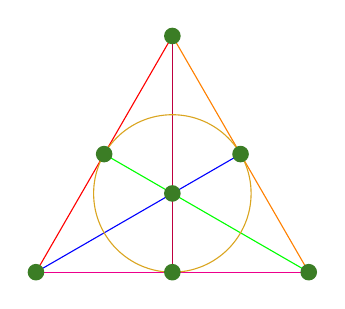
\begin{tikzpicture}
  \draw[color = blue] (30:1)  -- (210:2);
  \draw[color = green] (150:1) -- (330:2);
  \draw[color = purple] (270:1) -- (90:2);
  \draw[color = red] (90:2)  -- (210:2);
  \draw[color = magenta] (210:2) -- (330:2);
  \draw[color = orange] (90:2)  -- (330:2);
  \draw[color = Goldenrod] (0:0)   circle (1);
  \fill[color = OliveGreen] (0:0)   circle(3pt)
        (30:1)  circle(3pt)
        (90:2)  circle(3pt)
        (150:1) circle(3pt)
        (210:2) circle(3pt)
        (270:1) circle(3pt)
        (330:2) circle(3pt);
\end{tikzpicture}
\end{center}


\end{frame}

\begin{frame}{Colourability}
\begin{deff}
An $ m $-colouring of the hypergraph $ H = (V,E) $ is a partition in $ m $ subset of $ V = U_1 \sqcup ... \sqcup U_m $ such that for every edge $ \beta \in E $ we have $ \beta \not \subseteq U_i $ for all $ i = 1, ... , m $. A hypergraph $ H $ is $ m $-colourable if there exists a proper $ m $-colouring.
\end{deff}




\begin{figure}

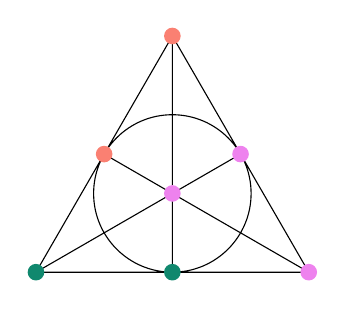
\begin{tikzpicture}

  \draw (30:1)  -- (210:2)
        (150:1) -- (330:2)
        (270:1) -- (90:2)
        (90:2)  -- (210:2) -- (330:2) -- cycle
        (0:0)   circle (1);
  \fill[color = Violet] (0:0)   circle(3pt) ; 
  \fill[color = Violet] (30:1)  circle(3pt);
  \fill[color = Salmon]     (90:2)  circle(3pt);
   \fill[color = Salmon]     (150:1) circle(3pt);
   \fill[color = PineGreen]     (210:2) circle(3pt);
   \fill[color = PineGreen]     (270:1) circle(3pt);
   \fill[color = Violet]     (330:2) circle(3pt);
\end{tikzpicture}
\caption{A 3-colouring for the Fano Plane}
\end{figure}

\end{frame}

\begin{frame}{Coverability}


\begin{deff} \label{def:cover}
A hypergraph $ H = (V,E) $ is said \textit{$ c $-coverable} if there exists a partition in $ c $ subset of $ V = U_1 \sqcup ... \sqcup U_c $ such that every $ U_i $ is a \textbf{vertex cover}, which means  that for all $ \beta \in E $ we have $ \beta \cap U_i \neq \emptyset $.
\end{deff}
\begin{figure}

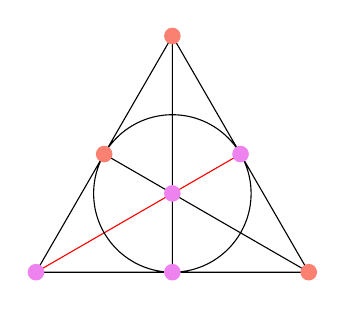
\begin{tikzpicture}
  \draw[color = red] (30:1)  -- (210:2);
  \draw      (150:1) -- (330:2)
        (270:1) -- (90:2)
        (90:2)  -- (210:2) -- (330:2) -- cycle
        (0:0)   circle (1);
  \fill[color = Violet] (0:0)   circle(3pt) ; 
  \fill[color = Violet] (30:1)  circle(3pt);
  \fill[color = Salmon]     (90:2)  circle(3pt);
   \fill[color = Salmon]     (150:1) circle(3pt);
   \fill[color = Violet]     (210:2) circle(3pt);
   \fill[color = Violet]     (270:1) circle(3pt);
   \fill[color = Salmon]     (330:2) circle(3pt);
\end{tikzpicture}
\caption{Steiner System $S(2,3,v)$ for $ v>3 $ are not $ 2 $-coverable}
\end{figure}
\end{frame}

%\begin{tikzpicture}
%  \draw (0,0)  -- (3,0) -- (3,3) -- (0,3) -- cycle;
%
%  \fill[color = Violet] (0,0)   circle(3pt) ; 
%  \fill[color = Violet] (0,3)  circle(3pt);
%  \fill[color = Salmon]     (3,3)  circle(3pt);
%   \fill[color = Salmon]     (3,0) circle(3pt);
%   \fill[color = Violet]     (0,1.5) circle(3pt);
%   \fill[color = Violet]     (1.5,1.5) circle(3pt);
%   \fill[color = Salmon]     (1.5,0) circle(3pt);
%\end{tikzpicture}

\begin{frame}{Cover ideal}
For an hypergraph $ H = (V,E) $ with $ V = \{ x_1, ... ,x_v\} $ consider the polynomial ring $ k[V] = k[x_1, ... ,x_v] $:
\begin{deff}
The \textbf{cover ideal} of the hypergraph $ H $ in $ k[V] $ is:
\begin{equation*}
J(H) := \left\langle x_{j_1} \cdots x_{j_r} \,|\, \{ x_{j_1} , ... , x_{j_r}\} \text{ is a vertex cover of } H \right\rangle  = \bigcap_{\beta \in E} \p_\beta
\end{equation*}
\end{deff}
Where for every hyperedge $ \beta = \{ x_{i_1} , ... , x_{i_r}\} \in E  $ then $ \p_\beta $ is the prime ideal $ \left\langle  x_{i_1} , ... , x_{i_r} \right\rangle  $
\end{frame}


\begin{frame}{Coverability and containment}
For a hypergraph $ H = (V,B) $ we define $ \tau (H) $ as $ \min_{\beta \in B} \{ |\beta |\}$, so we obtain:
\begin{teo}[Theorem 4.8 of \cite{Bal21Steiner}] \label{teo:col:cont}
Let $ H = (V,B) $ be a hypergraph, if $ H $ is not $ d $-coverable then 
\[ J(H)^{(\tau(H))} \not \subseteq J(H)^d \]
\end{teo}
For example for Steiner Systems we have:
\begin{prop}[Proposition 4.9 of \cite{Bal21Steiner}]
If $ v>3 $ and $ S = (V,B) $ is a Steiner Triple System $ S(2,3,v) $, then $ J(S)^{(3)}  \not \subseteq J(S)^2$
\end{prop}
\end{frame}

\begin{frame}{Colourability and containment}
\begin{teo} \label{teo:borin1}
	Consider a simple hypergraph $H = (V,B)$, if we indicate $\tau = \tau (H)$ and the cover ideal $ J = J(H)$,  then for all $ q \leq |V|$ if $ H $ is not $ q $-colourable then we have: 
%	\begin{enumerate}
%	\item $ \mm_V^{q-1} \in J(H)^{( \tau (q-1) )} $
%	\item 
 \[J^{( \tau(q-1) )} \not \subseteq J^q \]
%	\end{enumerate}
\end{teo}
\end{frame}

\begin{frame}
The proof rely on the two results:
\begin{teo}[Theorem 3.2 of \cite{Fran10Colourings}] \label{teo:col:chi}
Let $ H = (V,E) $ be a simple hypergraph on $ V = \{ x_1 , ... , x_v\} $, then for all $ d >0 $ we have $ (x_1 \cdots x_v)^{d-1} \in J(H)^d $ if and only if $ d \geq \chi(H) $, where $ \chi(H) $ is the minimum integer $ c $ such that $ H $ is $ c $-colourable
\end{teo}
\begin{prop}\label{teo:sym_radical}
If $ I $ is a radical ideal in a polynomial ring we have:
\begin{equation}
		I^{(m)} = \bigcap_{\p \in \Ass(R/I) } \p^m
	\end{equation}
\end{prop}
\end{frame}

\begin{frame}[allowframebreaks]{Bibliografia}
			\printbibliography[heading=none, notcategory=fullcited]	
\end{frame}

\end{document}
